\documentclass{article}
\begin{document}

The spin independent proton-LKP cross sections following from the effective interaction Lagrangian \ref{lagrangianq}+\ref{lagrangiang} will be:

\begin{equation}
    \sigma_{SI}=\frac{\mu^2}{\pi}\left(\frac{f_p}{m_\kga}\right)^2
\end{equation}

$\mu=\frac{m_\kga m_p}{m_\kga+m_p}$ being the reduced mass of the proton-LKP system. The effective four point coupling $\frac{f_p}{m_\kga}$ is given by \ref{effcoup}.  

The scalar quark contribution to the spin independent  effective coupling gets contributions from the Higgs exchange diagram and the KK-quark exchange diagrams labeled with a superscript: 
\begin{equation}
    f_q^h=(g m_w \frac{s_w^2}{c_w^2} \cos^2(\theta_w^{(1)}) + g m_w \sin^2(\theta_w^{(1)}))\frac{\lambda_q}{m_qm_h^2}
\end{equation}

\begin{equation}
  f_q^q=-g_{\kga q\kq}^2\frac{5m_\kga^2-m_\kq^2}{(m_\kga^2-m_\kq^2)^2}  
\end{equation}

The spin independent quark-DM effective coupling also get a a quark-twist-2 contribution:

\begin{equation}
    g_q=-g_{\kga q\kq}^2\frac{4}{(m_\kga^2-m_\kq^2)}
\end{equation}

Finally the gluon contribution:

\begin{equation}
    f_g=(g_v^2C_{1v}+g_a^2C_{1a}+(g_v^2+g_a^2)\frac{B_6m_n^2}{m_\kga^2})\frac{1}{36\pi m_\kga^2}
\end{equation}

where $C_{1v},C_{1a} \text{and} B_6$ are Passarino-Veltmann coefficients given in the Appendix  

The spin dependent proton-LKP cross section are given by:

\begin{equation}
    \sigma_{SD}=\frac{\mu^2}{\pi}\sum_{R,L}\sum_{q=u,d,s}\left(\frac{\Delta q_p}{4(m_\kga^2-m_\kq^2)}\right)^2
\end{equation}
where the first sum runs over right-handed and left-handed external quarks.


%\begin{equation}
%    g_{\kga\kga h}=g m_w \frac{s_w^2}{c_w^2} \cos^2(\theta^{(1)}) + g m_w \sin^2(\theta^{(1)})
%\end{equation}

\subsection{comparison with earlier results}

The effective 4-point couplings and proton-DM elastic cross sections have been preformed by Hisano et al. \cite{1012}.  They calculated the cross sections using the radiative corrections from \cite{oldcorrections}, apporximated the LKP by the hyper-charge boson  $B^{(1)}_\mu$ and for the spin dependent cross section assumed SM masses were negligible and all KK-masses except the LKP were degenerate using the splitting between the LKP and the other KK-particles as a free parameter.  Figure \ref{si1012} Shows a comparison between \cite{1012} and the DarkSUSY routine using the same approximations, which suggest a good correspondence. 


\begin{figure}[H]
    \centering
    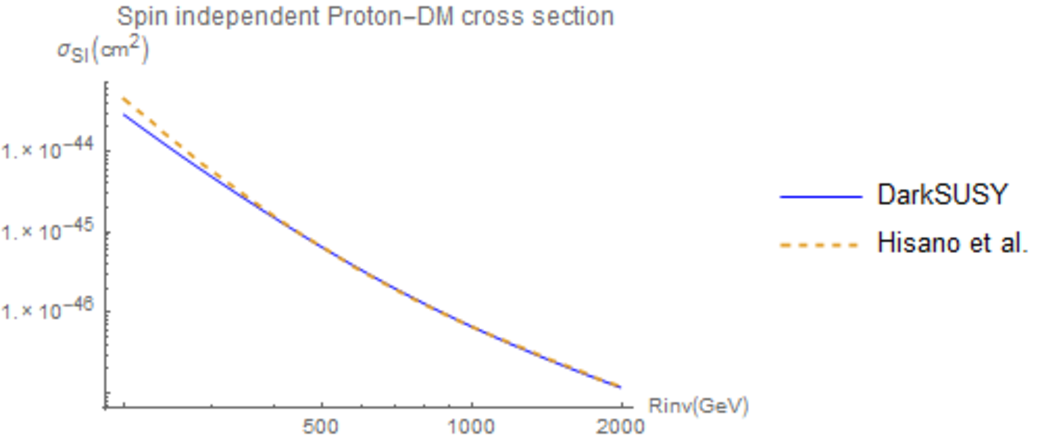
\includegraphics{SI1012.pdf}
      \caption{Comparison of the spin independent cross section obtained using DarkSUSY and \cite{1012}}
    \label{si1012}
\end{figure}

\begin{figure}[H]
    \centering
    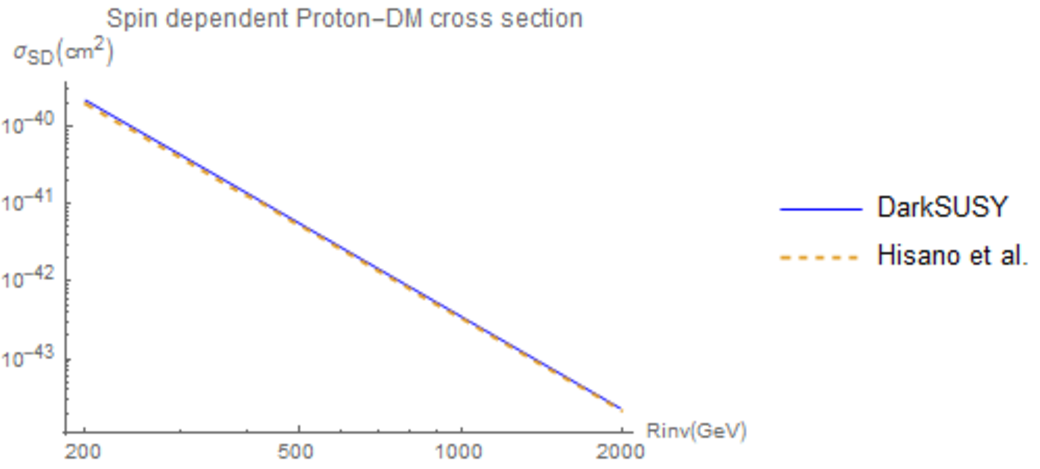
\includegraphics{SD1012.pdf}
    \caption{Comparison of the spin independent cross section obtained using DarkSUSY and \cite{1012}}
    \label{SD1012}
\end{figure}

\subsection{mUED cross sections}
In figure \ref{SI52050l} the spin independent cross sections calculated in mUED  using the full radiative correction are shown for different choices of $\Lambda$. Choosing a larger cutoff relaxes the degeneracy though radiative correction thereby reducing the cross section as all contributions except $f_q^h \ $ are inversely proportional to the mass splitting. For larger $R^{-1} \ $ the choice of $\Lambda$ is less important as $f_q^h \ $ dominates this regime as shown in figure \ref{couplingcontribution}. 


SI: $4\cdot10^{-47}-2\cdot10^{-47} \ $ for $\Lambda R=20,50$ 

SD: $6\cdot10^{-44}-2\cdot10^{-44} \ $ for $\Lambda R=20$

SD: $4\cdot10^{-44}-\cdot10^{-44} \ $ for $\Lambda R=20$
\begin{figure}[H]
    \centering
    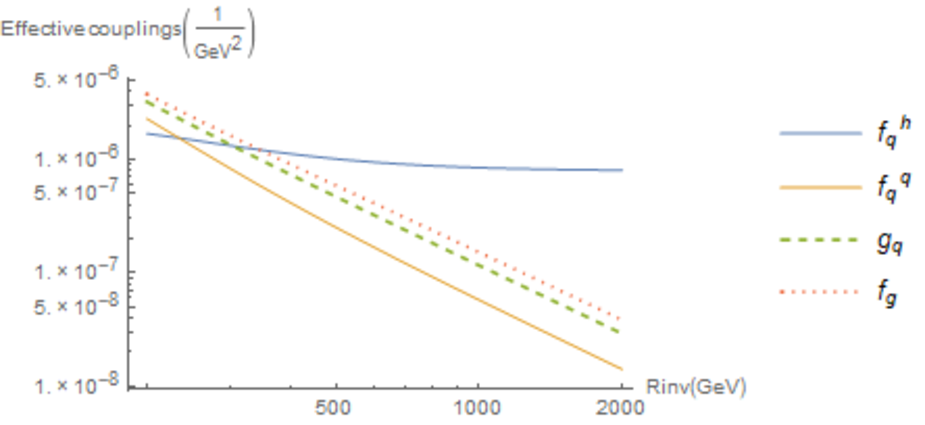
\includegraphics{cuoplingcontrib.pdf}
    \caption{}
    \label{couplingcontribution}
\end{figure}
\begin{figure}[H]
    \centering
    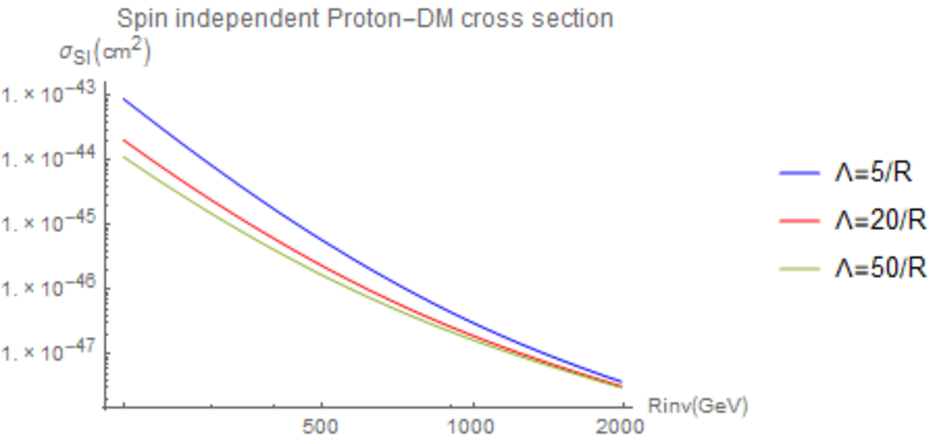
\includegraphics{SI52050.pdf}
    \caption{}
    \label{SI52050l}
\end{figure}
\begin{figure}[H]
    \centering
    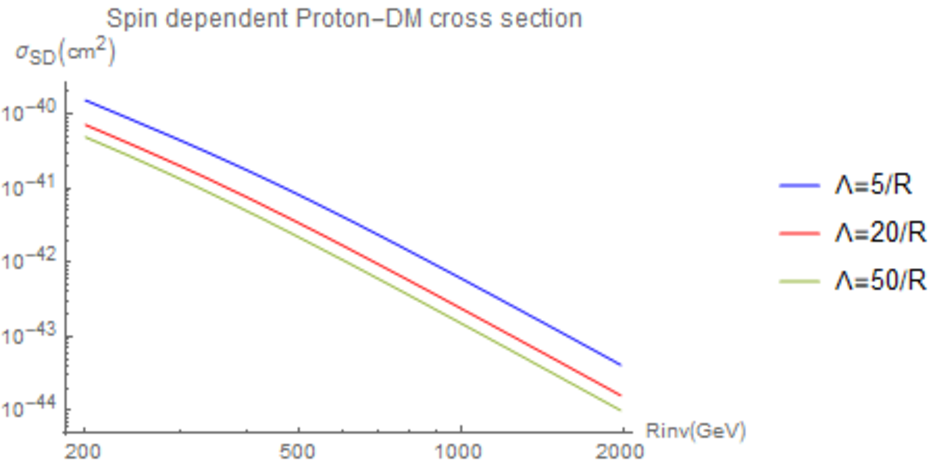
\includegraphics{SD52050.pdf}
    \caption{Caption}
    \label{fig:my_label}
\end{figure}

\subsection{nonminimal effects}

Figure \ref{daqsi} shows the spin independent cross sections of the KK-photon with the proton. Here the mass splitting $\Delta_q=\frac{m_\kq-m_\kga}{m_\kga}$ has been varied from 0.02 to 0.5 for all quarks excluding the top-quarks. The cross section is enhanced as the KK-quarks and the KK-photon become degenerate, although this enhancement is slower than the one found by \cite{1012}. 

As the degeneracy is lifted, i.e $\Delta_q$ is increased, the cross sections saturate as $f_q^h \ $ does not depend on $\Delta_q$ whereas the other contributions are inversely proportional to $\Delta_q$. Therefore when $\Delta_q$ is sufficiently large only $f_q^h \ $ is the only relevant contribution. This saturation happens faster for larger $R^{-1} \ $ as $f_q^h \ $  only depends on $R^{-1} \ $  through radiative corrections, while all other contributions scale as $R^{-2} \ $. The spin dependent cross sections are shown in figure \ref{daqsd} for completeness. 


\begin{figure}[H]
    \centering
    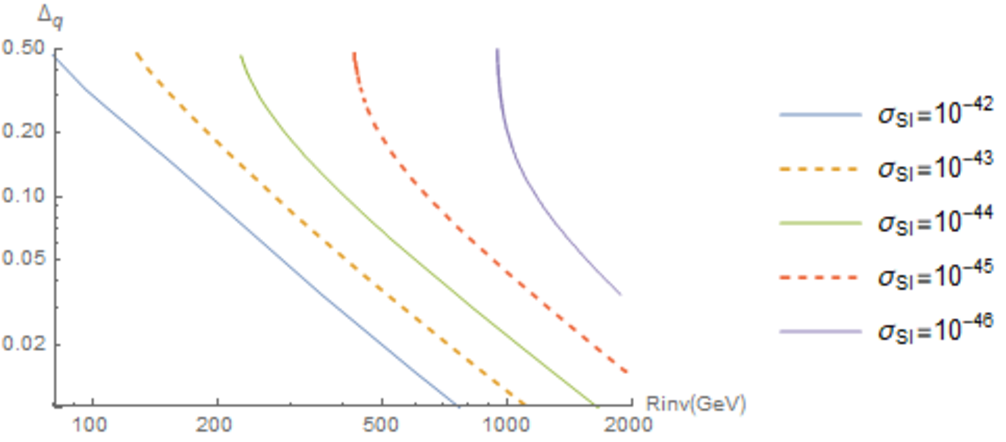
\includegraphics{deltaqSI.pdf}
      \caption{Spin-independent cross section with a proton in the degeneracy $\Delta_q=\frac{m_\kq-m_\kga}{m_\kga}$, $R^{-1}$ plane were the degeneracy was fixed for all quarks except the top-quark}
    \label{daqsi}
\end{figure}
\begin{figure}[H]
    \centering
    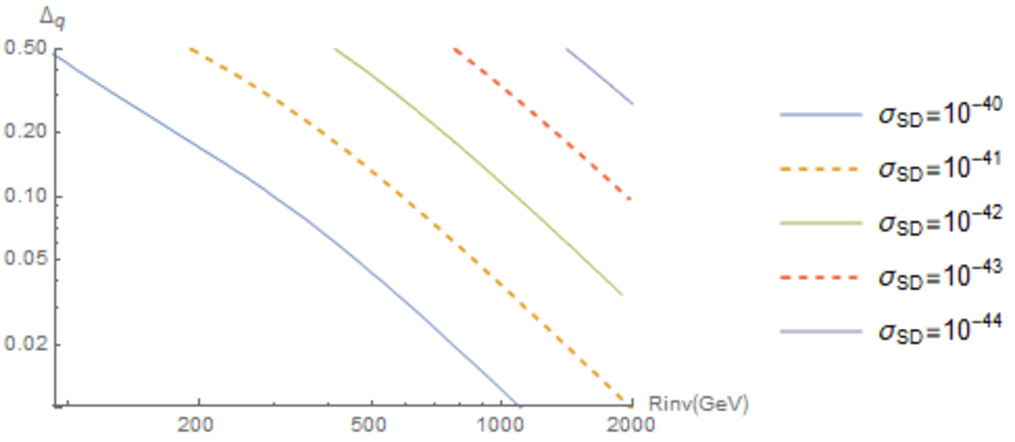
\includegraphics{deltaqSD.pdf}
      \caption{Spin-dependent cross section with a proton in the degeneracy $\Delta_q=\frac{m_\kq-m_\kga}{m_\kga}$, $R^{-1}$ plane were the degeneracy was fixed for all quarks except the top-quark}
    \label{fig:my_label}
\end{figure}

When we instead fix the mass of one KK-quark figure \ref{dudsi} and \ref{dssi} we again find the cross sections are enhanced for values of $\Delta_q$ below the mUED value, the enhancement is not as strong as in figure \ref{daqsi}.  For values of $\Delta_q$ above the mUED value the cross sections 
again become independent of $\Delta_q$, however the saturation already starts around $\Delta_q=0.1$ and the cross sections tend towards larger values than in  figure \ref{daqsi}, The difference however is smaller for larger $R^{-1} \ $ with the $10^{-46}\text{cm}^2$ contours being almost identical for $\Delta_q$ larger than the mUED value regardless of whether we fixed the mass of an up-,down- or strange-quark or all KK-quarks.   

There is no appreciable difference between varying the degeneracy of an up-, down-, or strange-quark so long as $\Delta_{u/d/s}>0.1$.


\begin{figure}[H]
    \centering
    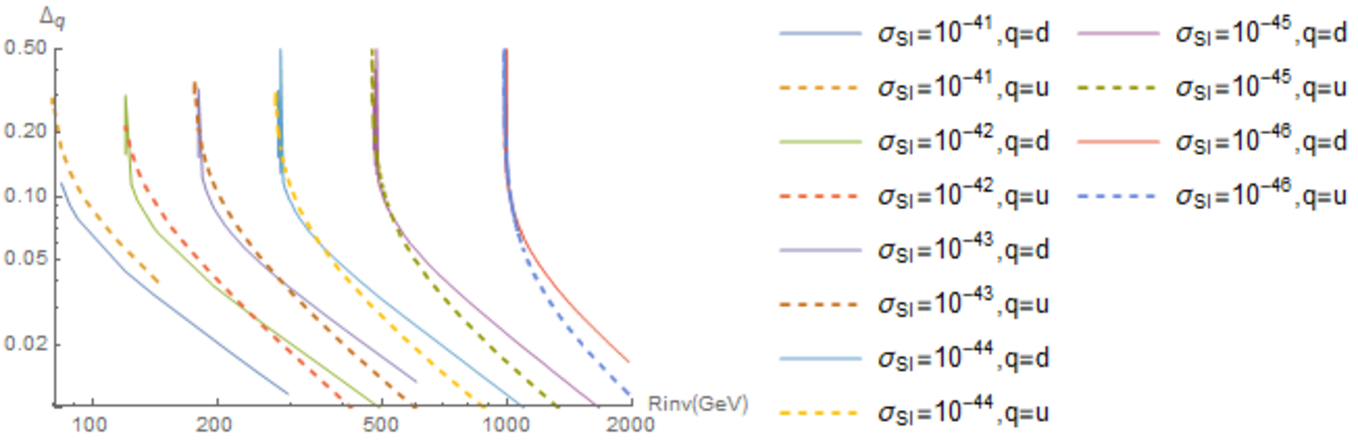
\includegraphics[width=\textwidth]{deltaudSI.pdf}
      \caption{Spin-independent cross section with a proton in the degeneracy $\Delta_q=\frac{m_\kq-m_\kga}{m_\kga}$, $R^{-1}$ plane were the degeneracy was fixed for the down-quark(filled lines) or up-quark(dashed lines) while all others kept mUED values}
    \label{dudsi}
\end{figure}\begin{figure}[H]
    \centering
    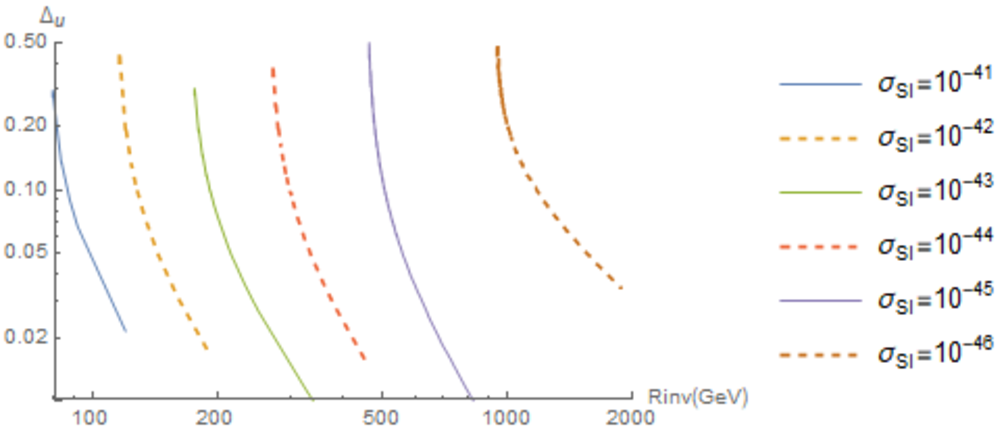
\includegraphics{deltasSI.pdf}
      \caption{Spin-independent cross section with a proton in the degeneracy $\Delta_q=\frac{m_\kq-m_\kga}{m_\kga}$, $R^{-1}$ plane were the degeneracy was fixed for the strange-quark while all others are kept mUED values}
    \label{dssi}
\end{figure}



\subsection{Effect of finite corrections}
Here we compare the cross sections calculated using only mass correction proportional to $\ln(\frac{\Lambda}{R^{-1}})$ which were calculated in \cite{oldcorrections} and the cross sections calculated using mass correction from \cite{freitas2018radiative} which include finite corrections.Figures \ref{simasshow12} and \ref{sdmasshow12} show the spin independent and spin dependent cross sections respectively with and without finite corrections with $\Lambda=\frac{20}{R}$. 

For the spin independent cross section  finite corrections are less important for large $R^{-1} \ $ as shown in \ref{relimp}, as $f_q^h \ $, which does not depend on the KK-masses, dominates in this region. However the finite contributions still cause up to 20\% decrease in the allowed parameter region.

The spin dependent cross sections are significantly reduced by including finite corrections as they increase the mass splitting of the KK-quarks and KK-photons.  

 
\begin{figure}[H]
    \centering
    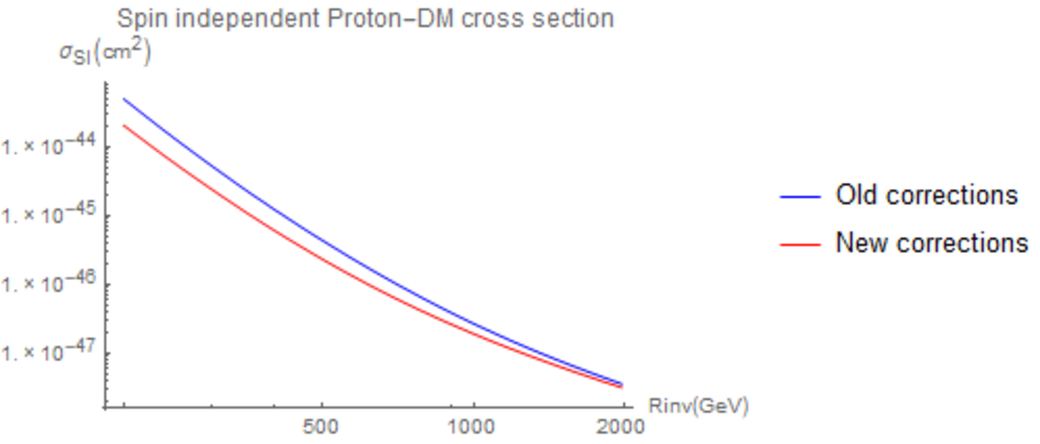
\includegraphics{SImasshow12.pdf}
    \caption{Caption}
    \label{simasshow12}
\end{figure}
\begin{figure}[H]
    \centering
    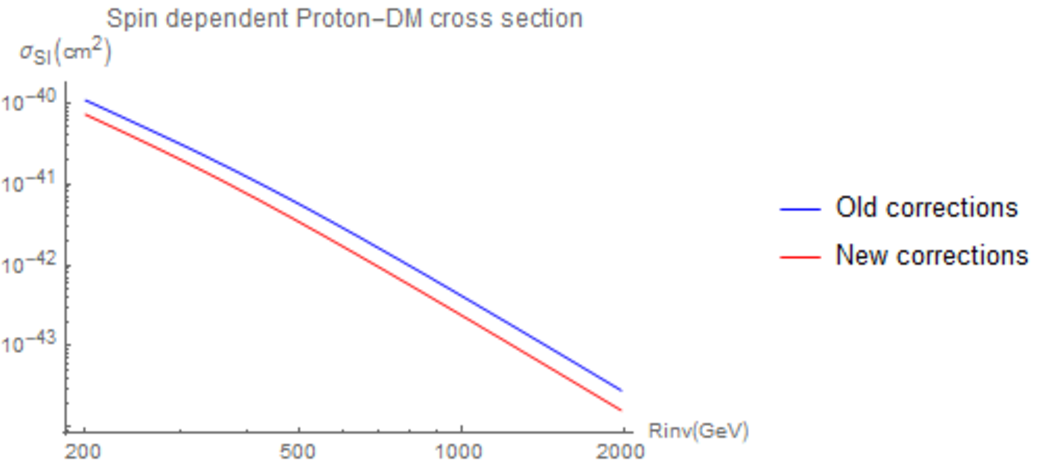
\includegraphics{SDmasshow12.pdf}
    \caption{Caption}
    \label{sdmasshow12}
\end{figure}
\begin{figure}[H]
    \centering
    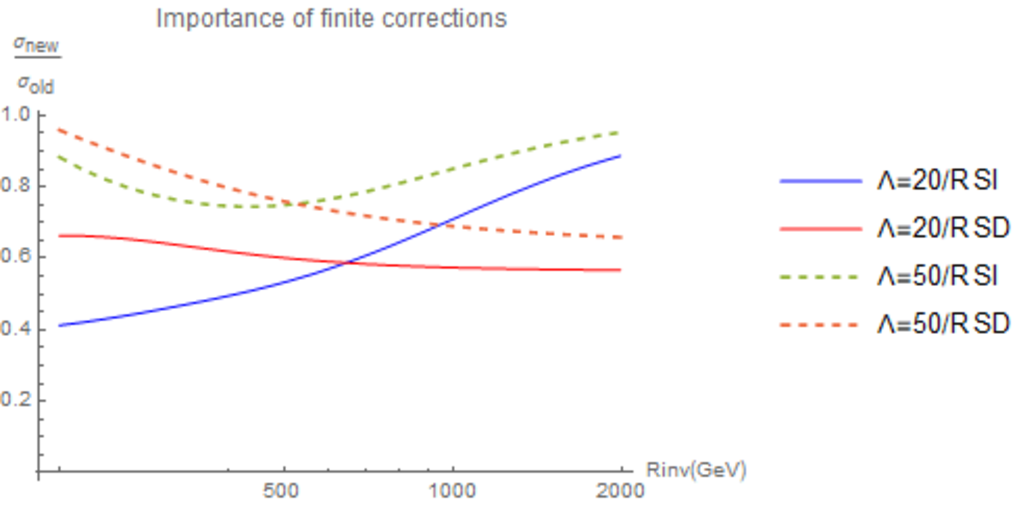
\includegraphics{relimp.pdf}
    \caption{Caption}
    \label{relimp}
\end{figure}


\end{document}